\chapter{Introduction}

\section{Context}

This thesis is the capstone project of my master's program, between the academic years 2019-2021 at MIT Media Lab, where I am a Research Assistant at the groups Opera of the Future and Future Sketches.

The work presented here has been developed mostly working remotely during the COVID19 pandemic, while at home in Boston MA.

\begin{figure}[h]
	\centering
	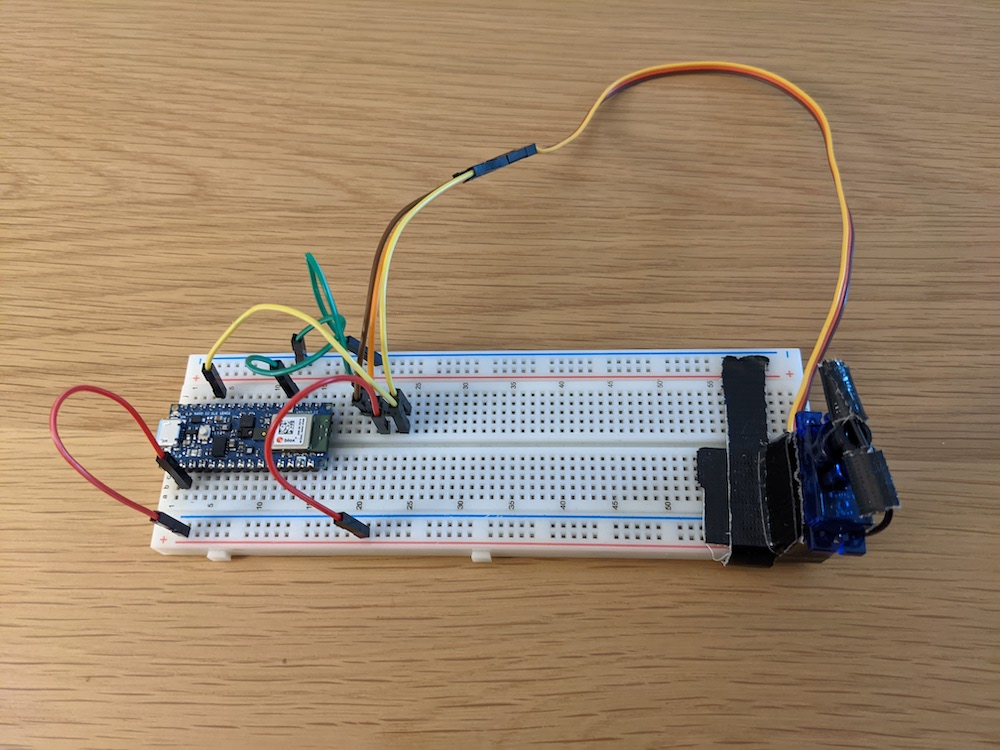
\includegraphics[width=0.75\textwidth]{images/desk.jpg}
	\caption{Desk at home}
	\label{fig:desk}
\end{figure}

This thesis is a collection of media arts instruments, using tiny machine learning, and with a strong emphasis on digital ethics and Do-It-Yourself (DIY). Its main audience is beginners and artists, and it is my hope that this work can inform the discourse and practice of a new generation of artists,  designers, educators, programmers, policy makers, activists, and enthusiasts.

Machine learning can be really difficult and often relies on proprietary software and hardware. They often need to be trained in borrowed and rented resources, such as the service Google Colab, which allows you to share and train ML models on the cloud. This thesis shows users how to build machine learning art systems that can circumvent this and allow for more control of their data.

Artists have an unprecedented access to new tools for making new tools and instruments, and this thesis intends to be a foundation for a new generation of instruments for manipulating audiovisual material, using machine learning. This approach is really exciting because it allows beginners and artists to train their instruments instead of programming them, by inputting data for tuning, instead of having to write lines of code and fixed thresholds for changing their behavior.

Machine learning algorithms are written by humans, and then trained on biased data, and they are deployed to the world, where they affect our lives. These imperfections are highlighted over the course of this thesis, by being explicit about the assumptions and quantizations performed when working with data.

TODO: Add example of biased dataset that is commonly used.

The proliferation of surveillance tools and now of microcontrollers allows for an even more pervasive surveillance and data leaks by governments and corporations. This thesis allows for beginners and artists to develop their own databases, by self sensing and surveillance. TODO: explain self-sensing and surveillance, and explain harms of surveillance, with an example.

Low power and repurposable
Tiny machine learning is defined as machine learning performed with low-power devices TODO: add citation or mention that it is my own definition. The proposal of media arts instruments that can run on little power, rechargeable batteries is a friendly use of resources for experimentation in arts. This is in contrast with the high power use and critique of other emerging fields such as Non Fungible Tokens (NFTs) and cryptoart. The proposal of these scriptable open source instruments allows for users to continuously tweak and modify their instruments, repurpose the hardware, and enable sharing.

TODO: Add a reference to an early tiny ML paper.

\section{Objectives}

With the release of TensorFlow Lite Micro, the TinyML Foundation, new avenues have been opened for creative expression using machine learning in microcontrollers.

TODO: Explain what is TensorfLow Lite Micro, what does it do, the same for TinyML Foundation

COMMENT: add in a paragraph here that combines the points you make in the first paragraphs -> the main contributions of YOUR thesis... which it seems is basically just addressing a bunch of the context section? Blakeley Payne's thesis does a good job of outlining contributions. It's also good to do here to understand where you are going

Homebrew examples, teach people how to build their own databases, and how to circumvent corporations view,

TODO: Terms and conditions comic book. If people were to read terms and conditions, it would take them X years

You can train an instrument to only detect your voice, your accent, your living conditions.

TODO: add blurb main inspiration about trail building and skatepark, and playpens, sandbox

TODO: add Marina Berry’s paper on playgrounds, child development

TODO: Technology and Public Art with Rafael Lozano-Hemmer | June 3, 2020
https://www.youtube.com/watch?v=QgVdEmqmuEE
36m28s
Rafael Lozano-Hemmer: “Face recognition needs to be banned in all applications except art.”

TODO: add Zoom example of garbage speech to text
TODO: Add in a glossary of terms to go over the basics of machine learning
TODO: Add contextual stories to frame each aspect
TODO: More pictures
TODO: Add how everything is public, even the errors
TODO: Raspberry Pi example, it’s cheap but it needs a lot of extra hardware to be used
TODO: Also add examples about April Fools Day and Terms and Conditions, about owning your soul
TODO: link https://www.youtube.com/watch?v=jOQ-9S3lOnM\&t=125s
TODO: Terms and conditions citation: (copied this in from my thesis, but check out McDonald and Cranor 2008) https://kb.osu.edu/handle/1811/72839 "Just considering privacy policies shown to people online in one year, it's been estimated that consumers would need approximately 244 hours to read, not skim, privacy policies shown to them in one calendar year."


\section{Outline}

This thesis will cover the following chapters:

\begin{enumerate}
        \item Chapter 2: Background: the inspiration and context of this thesis. TODO: add literature that informs my work.
    \item Chapter 3: Early experiments: my earlier work that led to this thesis, in the topics of media arts education, microcontrollers, and machine learning.
    \item Chapter 4: Tiny Trainable Instruments: description of design strategies for the software and hardware, description of the support team working on this thesis.
    \item Chapter 5: Project evaluation: user feedback, field notes.
    \item Chapter 6: Future work: next iterations of the instruments, and their proposed use for educators and artists.
  \end{enumerate}
